\documentclass[conference]{IEEEtran}
% \IEEEoverridecommandlockouts
% The preceding line is only needed to identify funding in the first footnote. If that is unneeded, please comment it out.
\usepackage{cite}
\usepackage{amsmath,amssymb,amsfonts}
\usepackage{algorithmic}
\usepackage{graphicx}
\usepackage{textcomp}
\usepackage{xcolor}
\graphicspath{ {./results-final/} }

\usepackage{rotating}
\usepackage{xparse}
\usepackage{booktabs, makecell, multirow}
\NewExpandableDocumentCommand\mcc{O{1}m}
    {\multicolumn{#1}{c}{#2}}
\usepackage{siunitx}
%\def\BibTeX{{\rm B\kern-.05em{\sc i\kern-.025em b}\kern-.08em    T\kern-.1667em\lower.7ex\hbox{E}\kern-.125emX}}


\begin{document}

\title{Where we're going, we don't need (negative) labels}

\author{David~J.~Elkind, Chief Data Scientist, DNSFilter}

\maketitle

\begin{abstract}
    Weakly supervised methods can train highly effective machine learning models for computer security, even when benign labels for data are entirely missing. Typically, computer security data only contains labels for the ``bad stuff" (malware, botnet domains), whereas labels for the ``good stuff" are either missing entirely, or only cover trivial cases (Microsoft software, Alexa Top 1 Million Domains). The standard supervised classification approach requires all samples to have a label. However, it can be very expensive and time-consuming to obtain a large, diverse sample benign labels. Using two publicly-available datasets, \textsc{ember} and Namgung's DGA corpus, we show that weakly-supervised learning methods out-perform conventional supervised learning when one class is unlabeled (a mix of positive and negative data in some unknown proportion). Moreover, we show that applying conventional supervised learning approaches to unlabeled data creates a ``backdoor" in the machine learning model. We show that the weakly-supervised learning approach minimizes this vulnerability. Code is available at https://github.com/delkind-dnsf/camlis-2024-dont-need-neg-labels/
\end{abstract}

\begin{IEEEkeywords}
computer security, neural networks
\end{IEEEkeywords}

\section{Introduction}
    This paper proposes that \textbf{benign labels are not actually required to construct state-of-the-art machine learning models in computer security contexts}. Instead, advances in positive-unlabeled (PU) learning allow researchers to use unlabeled data (presumed to be a mix of benign and malicious data) to create robust and reliable machine learning models.

    We demonstrate the effectiveness of PU learning methods on two different computer security datasets. Our experiments show the effectiveness of PU learning methods directly by comparing models trained using a specific PU learning method to ordinary positive negative models which do not account for the semantic uncertainty inherent in unlabeled data. We construct synthetic positive-unlabeled datasets from real-world security data, and show that the chosen PU learning method produces high-quality models.

    The paper proceeds as follows. Section \ref{sec:background} gives background on how the PU learning problem arises in the computer security setting. Section \ref{sec:related} gives a brief overview of related work and outlines (TED)${}^n$, our chosen PU learning method. Section \label{sec:data} describes the two datasets used in this research, one for malicious domain names and one for malicious software. Section \ref{sec:results} describes the experiments and their results. Section \ref{sec:discuss} discusses the results and directions for future work and Section \ref{sec:conclude} concludes.


\section{Background}
\label{sec:background} 

    This paper is partially inspired by a pattern we observed at \textsc{camlis} 2023. Each and every \textsc{camlis} 2023 talk invariably contained an aside to the effect of ``...but as we all know, it's impossible to get labels for the benign data, so we had to improvise" and then the speaker would  explain an \textit{ad hoc} method or heuristic for labeling a large amount of data as (likely) benign. Then the speakers would apply a conventional positive-negative (PN) machine learning method to the known malicious and putatively benign data. 

    Let's take a step back and set the stage for supervised machine learning in computer security. The defining assumption of \textit{supervised} learning is that you have some objects and all of those objects have labels, and you want to build a model to assign the correct labels to as-yet-unseen objects. In computer security, these objects could be portable executable software, domain strings, abstract syntax trees, network packets, API calls, or other relevant computer security data. The labels are semantic categories; typically, these labels are simple binary categories, e.g. ``benign'' or ``malicious.'' Experts review the unlabeled objects to determine if they're malicious or not, but this process is time-consuming and expensive. Accordingly, computer security researchers frequently have datasets comprised of a small number of labeled samples examples on the one hand, and an enormous volume of unlabeled data on the other.

    That said, \textit{malicious} labels in particular are often widely available from threat feed subscriptions and similar services (e.g. VirusTotal or Hybrid Analysis for PE files, and Recorded Future or InfraGuard for Internet domains). However, the coverage of these services will always be incomplete. Moreover, the most effective adversaries will be very careful to evade detection. Thus, the fact that a PE file or domain name in a threat feed has not been labeled as malicious is not the same as positive proof that the domain is benign. It could simply be the case that its maliciousness has not yet been detected. In this way, even threat feeds, which are often seen as an authoritative resource for label in cybersecurity datasets, should be understood as source of PU labels, rather than PN labels.

    Naturally, expense of obtaining labels leads researchers to consider expeditious alternatives. So researchers seek some short-cuts, such as using heuristics, business rules or other imperfect substitutes for expert review. An alternative short-cut is to simply train a biased PN classifier, which \textit{ignores} unlabeled data problem and simply treats the unlabeled data as negatives. Naturally, this is a suboptimal solution. In this paper, we quantify the extent of that bias.

    But both of these approaches -- heuristic labels and training a biased model -- are is inherently unsatisfying, because the simplifying assumptions that underpin them become foundational components of the model. Any errors or sampling bias that these heuristics incur will distort the resulting model. These errors could cause the model to misclassify a malicious event as benign or \textit{vice versa}. In effect, heuristic labeling can create systematic security holes in the resulting model which originate in the labeling process itself. In the worst-case, the model may only learn to faithfully reproduce the rules or heuristics used to label the data as ``benign,'' leaving an exploitable backdoor for any malicious activity that deviates from the heuristics used to curate the benign data.

    By contrast, PU learning methods take a huge step forward for machine learning in computer security. \textbf{Weakly supervised methods can train highly effective binary classifiers, even though reliable labels for one of the classes are entirely missing.} PU learning does this by taking advantage of the enormous volume of \textit{unlabeled} data (presumably a mix of malicious and benign in some unknown proportion) that computer security practitioners are often able to passively collect.

    This paper will show the results of applying (TED)${}^n$ \cite{garg-2021}, an off-the-shelf PU learning method, to two different computer security problems using publicly available datasets. The first is malware classification using the \textsc{ember} dataset \cite{anderson-2018}. The second is malicious domain detection, comparing malicious domains produced by domain generation algorithms (\textsc{dga}) to benign domains (obtained from the Alexa Top Domains list) \cite{namgung-2021}.

    Both datasets include a large quantity of labeled, benign data. This is allows us to \textit{simulate} unlabeled data in a controlled fashion. We simply remove all the labels from the benign data and some fraction of the malicious data to create unlabeled data. Our experiments show that the PU learning models perform better the biased PN models when trained on the same data.

    Finally, the \textsc{ember} dataset also includes some unlabeled data. We simulate a dataset with a large portion of unlabeled data by treating all benign data and all unlabeled data as if they are unlabeled. We show that the (TED)${}^n$ classifier trained using this large set of unlabeled data is more effective than biased classifier that na{\"i}vely treats all unlabeled data as if it were the negative class.

\section{Related Work \& PU Learning}
\label{sec:related}

    Moving beyond the case of traditional classifiers, where all samples have labels, one encounters a variety of different ``weakly supervised'' paradigms, so named in contrast to the traditional ``strongly supervised'' approach. These weakly supervised methods include semi-supervised learning (where one has positive labels, negative labels and unlabeled data), noisy labels (where the data's labels are sometimes incorrect), unlabeled learning (where there are no labels at all), and complementary labels (where the label tells you what an object \textit{isn't}, but not what it \textit{is}). Examples of methods for all of these scenarios appear in \cite{mlws}.

    Despite its broad applicability to computer security problems, there is not an enormous literature base applying positive-unlabeled learning in this setting. Based on Google Scholar results for  academic publications that cite Garg \textit{et al.}, we believe that this paper is the first research to apply the (TED)${}^n$ method to cybersecurity data. Likewise, this paper is also the first to apply positive-unlabeled learning methods to either Namgung \textit{et al.}'s DGA dataset or Anderson \& Roth's \textsc{ember} dataset. Moreover, because these datasets are fully labeled, we can evaluate their true PN performance in a controlled manner, and study the models' performance as we vary the proportion of unlabeled data.

    In general, there is some literature applying various PU methods to computer security problems. Regarding PU learning for malware, in \cite{zhang-2019} the authors propose a cost-sensitive boosting method. And \cite{reddy-2020} ensembles some cost-sensitive several classifier types for the same purpose. As a framework, cost-sensitive learning and reweighted losses feature prominently in the PU literature; a number of similar concepts appear in \cite{mlws}. In the context of DGA, an example is \cite{fan-2022}, which introduces a novel PU learning method particularized to the unique dataset used in the paper.

    The widely-used nnPU method has also been applied to computer intrusion detection \cite{lv-2020}. 

    In this paper, we adopt the (TED)${}^n$ method of Garg \textit{et al}. Even though this method has limitations in its theoretical guarantees, we nonetheless adopt this method because it compares favorably to the other methods which we reviewed. The wide variety of methods surveyed in \cite{bekker-davis-2020} depend on unrealistic assumptions about the data, exhiibit sensitivity to hyper-parameters, or lack theoretical guarantees. Similarly, the kernel-based methods outlined in \cite{mlws} have theoretical guarantees, but kernel matrices do not scale favorably to large datasets, and the methods depend crucially on hyper-parameters for which tuning is impossible.

    Finally, the Garg \textit{et al.} paper shows that (TED)${}^n$ compares favorably to the nnPU method. The nnPU method proposed in \cite{kiryo-2017}, has a strong theoretical basis, does not have any hyper-parameters, is widely used, and it is often selected as a default method for PU learning tasks. However, nnPU requires one to know or obtain an mixture proportion estimate, which is not a trivial task. Moreover, Garg \textit{et al.} show that nnPU tends to under-fit relative to (TED)${}^n$, which is undesirable.

    (TED)${}^n$ is composed of two parts. The first part, best bin estimation (BBE), is used to estimate the proportion of positive samples among the unlabeled data. The second part, conditional value ignoring risk (CVIR), is a method to estimate a classifier from the positive-unlabeled data in a way that has lower bias than a model that na{\"i}vely treats the unlabeled data as negative data. Specifically, (TED)${}^n$ trains a biased binary classifier for 0 or more iterations, then computes the mixture proportion estimate using BBE applied to a held-out partition of the data, then removes the unlabeled samples with the greatest propensity to be positives from the training data, then trains a biased classifier for another iteration on the filtered data; this process is repeated until the training error converges. In combination, the method is able to \textit{simultaneously} estimate the mixture proportion and use that estimate to train a classifier by discarding the fraction of the unlabeled training data that are most likely to be positive. 

    The (TED)${}^n$ method is entirely agnostic to the nature of the classifier, requiring only that you can compute a loss value for each observation; therefore, (TED)${}^n$ method can accommodate data with many observations or features whenever the chosen machine learning model can. Finally, while the (TED)${}^n$ method does have a single hyper-parameter that's used to estimate the mixture proportion, our results do not vary much when it is adjusted. (We simply set is value to 0 in these experiments.)

    With respect to theoretical guarantees, (TED)${}^n$'s BBE method makes only modest assumptions about the data itself. The authors term this assumption the ``pure positive bin'' property, and it describes the case where that there is a threshold where only positive samples have model predictions larger than that threshold; moreover, this requirement can be relaxed with the introduction of a hyper-parameter. The authors provide theoretical guarantees that the mixture proportion estimator will be close to the true proportion with high probability.

    On the other hand, the authors do not provide theoretical guarantees for the CVIR method. Using the estimate of the proportion of positives among the unlabeled data, the CVIR method discards that same fraction of the unlabeled data that the model predicts as most likely to be positive. It is intuitive why the CVIR method might work -- if the model has an ability to differentiate among positives and negatives, then the unlabeled data that the model ranks as most likely to be positive will have the largest proportion of positives among them, and removing those samples implies that the remaining samples are largely negatives. That said, we would prefer some formal evidence that the improvement in model quality that we derive from omitting some of the positives among the unlabeled is greater than the \textit{degradation} in model quality that comes from the model mislabeling some \textit{negatives} and removing them. In a worst case, one can imagine a self-reinforcing scenario arising where the data removed from the training set causes the BBE method to become biased upwards, so that CVIR removes even more negatives from the unlabeled data, which worsens the quality of the BBE method, repeating \textit{ad nauseam.}

    We contrast (TED)${}^n$ to the biased PN classifier, which treats the unlabeled data as if it were actually all negative data. This is the simplest approach to training a machine learning model in the PU setting, because it simply ignores the core problem. However, the obvious flaw with this approach is that the model is more likely to misclassify test-time positive samples that are similar to one or more of the positive samples among the unlabeled data. We term these models ``biased classifiers'' for this reason. The extent of this bias will be greater or lesser depending on the proportion of positive samples among the unlabeled data.

\section{Datasets}
\label{sec:data}

    To demonstrate the generality of our chosen PU learning method to computer security applications, we apply the method to two datasets reflecting two distinct computer security problems. The first a corpus of domain strings labeled according to which malware family produced the string \cite{namgung-2021}. The second is \textsc{ember}, a corpus of portable executable (PE) files which are labeled as malicious, benign, or are unlabeled \cite{anderson-2018}. Both datasets are publicly available in Github repositories maintained by their respective authors.

    These datasets are not without limitations. Both datasets are somewhat old. Namgung et al. compiled their dataset prior to 2021, and \textsc{ember} was last updated in 2018. Their age doesn't particularly matter for this paper's experiments, which are solely about the relative efficacy of PU learning, but would matter a great deal if a person were to attempt to use the models developed in this paper as a security product.

    Additionally, both of these datasets are considered small by the standards of industrial computer security. In our professional work, a typical dataset is composed of hundreds of millions or even billions of observations. We state this to underscore the enormous burden of obtaining reliable labels of computer security artifacts at this scale, and highlight the role that PU learning plays in lessening that burden.

    Comparing the two tasks, we anticipate that malware classification will be more challenging than DGA detection. This is because DGA domains are characterized by their length and highly random, ``keyboard smash'' appearance. By contrast, legitimate websites tend to use  memorable words or short phrases as domain names. In particular, the models we use in this paper take the 3-grams of the domain as the input, so the model's task is simplified to assessing whether all of the 3-grams in combination look like more random strings or words.

    By contrast, PE files are binary files that have a rich structure and can be obfuscated in various ways to defeat security professionals attempts to detect them. Even detonating suspected malware is not foolproof, because malware authors can include techniques to detect if the program is operating inside of a sandbox and alter is behavior accordingly.

\subsection{Namgung's DGA Dataset}

    In computer security, malware authors often use DNS as a covert communications channel \cite{kuo-2023}. In a typical scenario, the malware author wishes to send instructions to or receive data from a compute that has been infected with the author's malware. Malware authors do not simply use an IP address coded into the malware for this traffic because it is fragile: blocking the IP address (e.g. via firewall) stops the communication. And authors do not use a single, pre-defined domain string for the same reason. Instead, malware authors will use some algorithmic method to procedurally and dynamically choose a domain string from among an enormous pool of possible domain strings. These are called domain-generation algorithms (DGA). The goal is to make it more challenging for security professionals to block this traffic because enumerating all possible domain names for that specific malware is challenging, and the malware author has the luxury of choosing which domains among the pool of possible domains that they wish to use for command and control of the malware.

    Namgung \textit{et al}.'s dataset of benign and DGA domains was collected with the intent of training a multi-class classifier to distinguish among different families of DGA domains \cite{namgung-2021}. The dataset is composed of 832,271 DGA samples and 603,387 benign domains. There is not an explicit test dataset, so we evaluate test-set metrics by using 5-fold cross-validation. In the present setting, we will use this dataset to build a binary classifier, collapsing all of the domains from different malware families into a single, positive class. 

    One limitation of  Namgung \textit{et al}.'s dataset is that its examples of benign domains are drawn from Amazon's Alexa Top One Million domain list. I've discussed the limitations of this approach elsewhere \cite{elkind-2023}, but I'll briefly recap them here.

    The main problem with using the most popular domain names as the negative set is that these domains are not likely to be at all similar to the types of domains to which one will be applying the machine learning model in the future. Alexa domains tend to be short, memorable, and often English-language dictionary words. There are hardly any punycode domains among them.\footnote{The DNS standard requires all domains to be written in ASCII characters. Punycode is an encoding scheme that allows any UTF-8 character to be represented using ASCII. This is necessary to correctly \textit{display} domains in languages that use non-ASCII characters, but ``under the hood'' the domain name is an ASCII string. For example, the domain g{\o}{\"o}g{\l}{\^e}.com is encoded as \texttt{xn--gg-fja0cj06b.com}.} Moreover, the concept of ``top domain" embodied in the Alexa list is limited solely to the domain names typed into a browser by users who have installed the Alexa extension. This leaves out the large volume of internet traffic that is not submitted to the address bar of a web browser (examples include e-mail clients, mobile social media applications, and internet-connected games).

    Moreover, if the goal of the machine learning method is simply to not block popular domains (\textit{vice} identifying malicious domains), one can do that with a whitelist without any need for machine learning. With this in mind, the real challenge of building an industrial protective DNS solution is that one will need to correctly handle traffic to obscure and newly-registered domains, and these domains may be markedly different from the most popular domains.


\subsection{Anderson \& Roth's \textsc{ember} Dataset}

    Our second computer security challenge is detecting malicious software (malware). Malware can take many forms, from key-loggers to trojans. Ransomware, which holds an organization's computers hostage until they pay the ransom, is the most prominent contemporary example \cite{crowdstrike-2024}.\footnote{The report discusses ransomware as a part of the threat landscape throughout, but the most conclusive statement of ransomware's future prospects can be found in this quotation ``Though CrowdStrike CAO assesses that ransomware will highly likely remain the primary extortion method through 2024, [big game hunting] adversaries will increasingly emphasize stolen-data exploitation as a means to pressure victims into payment.''} Inspecting a portable executable (PE) file for evidence that it may be malware is a standard feature of an antivirus solution or an endpoint security product. Anderson \& Roth compiled the \textsc{ember} dataset as a way to create a common benchmark dataset for detecting PE malware, much in the same way that \textsc{CIFAR} and ImageNet datasets are widely used in the computer vision literature. 

    As part of the same project, Anderson \& Roth also released software named \textsc{ember}, which is a feature extraction engine that transforms a PE file into a vector representation summarizing it. This is an important step because interpreting a binary composed of thousands or millions of bytes requires knowledge of which attributes are useful to measure from a security standpoint, and is the cornerstone for how a machine learning algorithm will make its risk assessments.

    Though the \textsc{ember} dataset and feature extraction engine are both somewhat dated (the latest version was released in 2018), it remains one of the only open datasets of PE software and open source feature-extraction engines.\footnote{Due to its age, we are forced to make two minor modifications to the feature extraction engine in order for it to work. The first is to increment the \texttt{lief} library (a free utility for parsing PE files) from 0.9 to 0.13. The second is fixing a bug that arises how recent versions of python handle computing the hash of an iterable. This bug is issue number 103 on the Github for \textsc{ember}. Both of these changes may alter the computed feature values.} The dataset contains 1.1 million PE files, and is partitioned into a training dataset (300,000 malicious, 300,000 benign and 300,000 unlabeled) and a test dataset (100,000 malicious and 100,000 benign).

\section{Experiments \& Results}
\label{sec:results}

    \begin{figure*}
        \centering 
        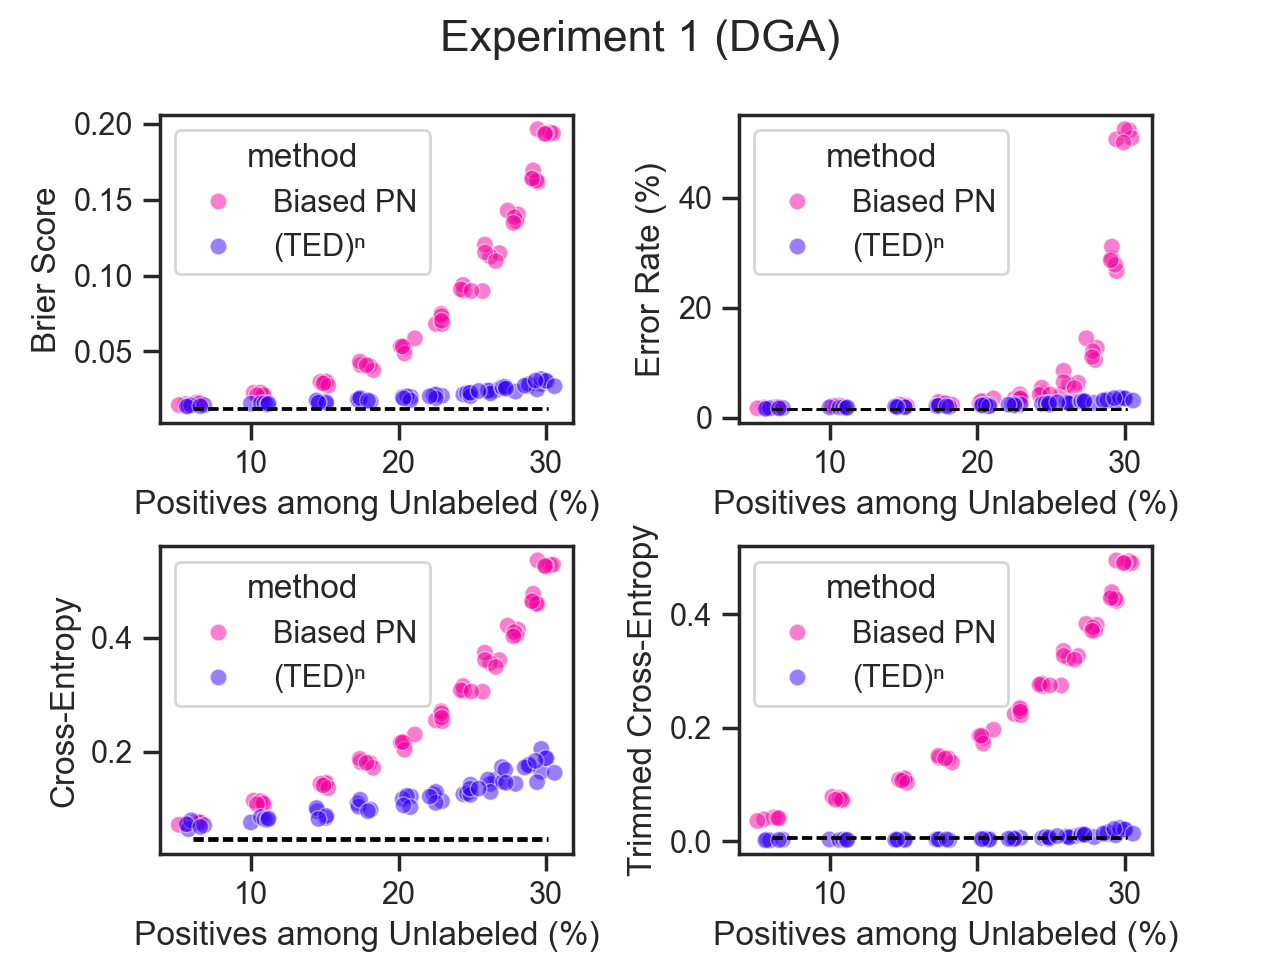
\includegraphics[scale=0.5]{experiment-1}
        \caption{Test-set metrics for experiment 1.} 
        \label{fig:exp1} 
    \end{figure*} 

    In these experiments, we compare the effectiveness of the (TED)${}^n$ procedure and a biased PN model trained on the same dataset, using the same models. The first two experiments simulate varying levels of mixture proportions among the unlabeled data by simulating unlabeled data. The first experiment does this for the DGA data, and the second for the \textsc{ember} corpus. We simulate unlabled data by removing a random portion of the positive samples from the positive set and adding them to the negative set, which we treat as unlabeled. A side-effect of this simulation is increasing the size of the unlabeled set decreases the size of the positive set and \textit{vice-versa}. The proportion of positives so relabeled varies from 5\% to 55\% in increments of 5\% (implying that the proportion of positives \textit{among the unlabeled} set varies between roughly 4\% and 35\%). This simulation allows us to assess the accuracy of the mixture proportion estimates, as well as how changing the value of the mixture proportion influences the efficacy of either training method. 

    The third experiment utilizes the unlabeled data from the \textsc{ember} corpus to directly compare the PU and biased learning scenarios. We do this by combining the negative class and the unlabeled data into a single unlabeled class and then applying the (TED)${}^n$ method. This experiment is closer to a real-world scenario where the true mixture proportion is unknown, because we are using data which is truly unlabeled we do not have any mechanism to monitor the efficacy of the (TED)${}^n$ method during training.

    In all cases, we report performance metrics on the test set. As a benchmark, we also report results for the traditional PN models trained without any augmentations made to their labels. These benchmark models characterize the ``best case'' scenario when one is blessed with a large, labeled dataset that does not reflect any label scarcity, labeling errors, nor inclusion of unlabeled data.

    In all cases, the model architectures and model hyper-parameters are identical for the benchmark models and experiments comparing PU learning and biased PN learning. Full model details are presented in appendix \ref{appendix:hyperparams}. Consequently, the only experimental variable is the training method used (either (TED)${}^n$ or a biased classifier). We measure four test-set metrics: Brier score, error rate, cross-entropy, and trimmed cross-entropy.\footnote{Trimmed cross-entropy is the same as the cross-entropy metric except it removes a fraction of the most extreme values before computing the average. This omission suppresses the influence of extreme values on the result, which can be very pronounced as there is no upper bound on the cross-entropy loss. Everywhere in this paper, the most extreme 2.5\% of values are removed from both the smallest and largest cross-entropy values; in total, 5\% of values are removed.}

    Finally, statistical results are presented in appendix \ref{appendix:tables}.

\subsection{Experiment 1: DGA Detection (simulating unlabeled data)}

    The purpose of Experiment 1 is to test whether applying the (TED)${}^n$ method to PU data for DGA domains produces a superior model compared to the na{\"i}ve method which treats unlabeled data as if it were negative data. 

    As a model, we use a feedforward multi-layer perceptron with residual connections. This network is essentially a tabular analogue composed of the residual blocks in \cite{he-2016}. The input to the model is the 3-grams of the reversed domain string. Reversing the domain string maintains adjacency of consecutive characters while enforcing that the top level domain (e.g. `.com') appears in a consistent location of the input, even when domains have varying lengths, and yields a modest improvement to the model.

    Figure \ref{fig:exp1} displays the results of Experiment 1. For each metric, a lower value indicates that the model is superior to a model with a higher value. The dashed horizontal lines indicate the ``gold standard'' benchmark for the PN classifier trained with perfect label information (no unlabeled data).\footnote{These lines technically display the upper and lower extremes of a 95\% confidence interval for the metric (computed from 5-fold cross-validation), but these intervals are narrow enough that they appear to be a single line in these figures.}

    The plots show a consistent pattern, wherein the (TED)${}^n$ method is often superior to the biased PN models. Moreover, discrepancy between the two methods is most pronounced when the proportion of positives among the unlabeled data is larger. This makes intuitive sense, because the PN method treats the unlabeled data as negatives, so when there are more positives in the unlabeled set, there is not a consistent signal to differentiate the two classes. Likewise, the (TED)${}^n$ and biased PN methods are most similar in performance when there is a smaller proportion of positives among the unlabeled data. However, even for small levels of label noise, the (TED)${}^n$ method displays superior Brier score and trimmed cross-entropy values. 

    A general trend is that the (TED)${}^n$ method produces models that are very close to the benchmark performance obtained by the traditional PN model without any label noise. The exception is the cross-entropy metric, which departs the benchmark performance, even though its values remain lower than the biased PN model. This is because the (TED)${}^n$ procedure tends to produce a small fraction of predictions which are \textit{very} incorrect. After removing these extreme values, the cross-entropy values are essentially indistinguishable from the benchmark performance across all levels of label noise.

    We use paired $t$-tests to test the null hypothesis that the difference in the paired means is zero against the alternative hypothesis that the distribution of (TED)${}^n$ results has a mean \textit{lower} than that of the biased PN model. These results are shown in table \ref{tab:exp1}. We carry out this test for each of the four metrics (Brier score, cross-entropy, error rate, and trimmed cross-entropy) for each percentage of positive samples treated as unlabeled data. In all instances but one, the results are statistically significant at the 5\% level. The exception is that the $t$-test reports no statistical difference in cross-entropy when only 5\% of the positives are moved to the unlabeled set. We conclude that (TED)${}^n$ provides an unambiguous benefit over a biased PN model when applied to the DGA task.

    \begin{figure*}
        \centering 
        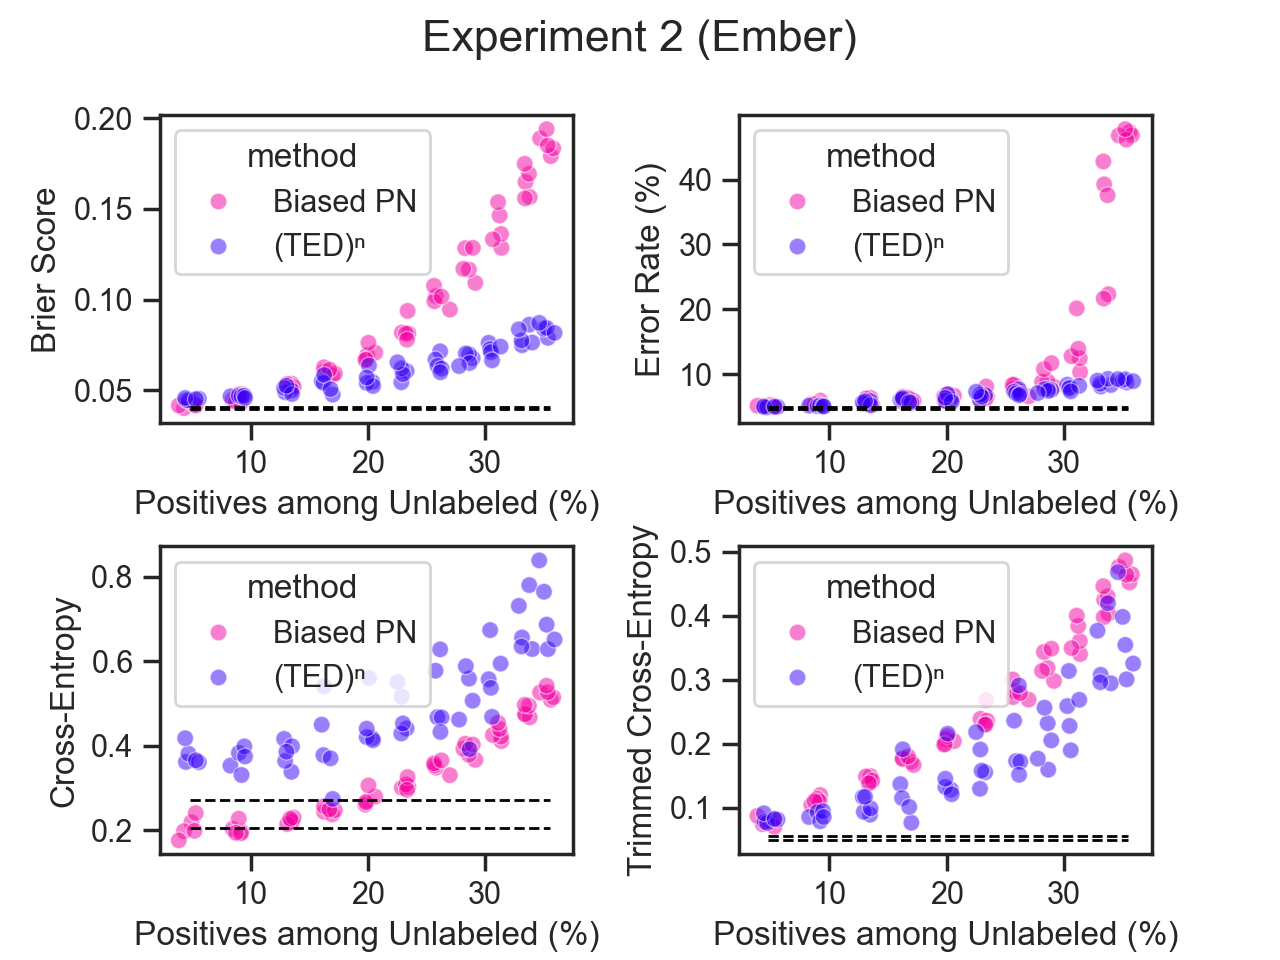
\includegraphics[scale=0.5]{experiment-2}
        \caption{Test-set metrics for experiment 2.} 
        \label{fig:exp2} 
    \end{figure*} 
\subsection{Experiment 2: Malware Detection (simulating unlabeled data)}

    
    Experiment 2 has the same design as Experiment 1, except that it is applied to the \textsc{ember} dataset. We do not utilize the \textsc{ember} dataset's unlabeled data in this experiment; this data is used in Experiment 3. Likewise, we use a similar feedforward multi-layer perceptron with residual connections. The input to the model is simply the \textsc{ember} feature vector; as a preprocessing step, inputs to the model are centered to have a mean of 0 and scaled to have a variance of 1. The estimates of the mean and variance are computed solely from the training data.

    Figure \ref{fig:exp2} displays the results of Experiment 2. As before, the dashed horizontal lines indicate the ``gold standard'' benchmark for the PN classifier trained with perfect label information (no unlabeled data), and these lines display the upper and lower 95\% confidence intervals for the metric (computed from 5-fold cross-validation).

    Overall, the results for Experiment 2 show that increasing the number of positives among the unlabeled data worsens both the (TED)${}^n$ model and biased PN model. Moreover, only error rate of the (TED)${}^n$ model is similar to the benchmark values, and only when the mixture proportion is small. That said, the  (TED)${}^n$ model still out-performs the biased PN model in terms of Brier score, error rate and trimmed cross-entropy.

    However, the cross-entropy results show that the (TED)${}^n$ model is consistently worse. We attribute this to the model giving a very incorrect prediction to a small fraction of samples in the (TED)${}^n$ model, and the losses on these samples are large enough to overwhelm the vast majority of instances which have a lower loss. This is confirmed by the trimmed cross-entropy results, which show that omitting these extremely large values usually lowers the average loss for the (TED)${}^n$ model below that of the biased PN model. In other words, it's not true that the (TED)${}^n$ model produces uniformly larger cross-entropy losses than the biased PN model for all observations; if it did, then the trimmed cross-entropy losses would show that the biased PN model has both lower cross-entropy and trimmed-cross entropy losses. 

    Additionally, the trend that (TED)${}^n$ has lower trimmed cross-entropy losses than the biased PN model is not universal. For each mixture value of the positives among the unlabeled data, there is one (TED)${}^n$ cross-validation fold which has a trimmed cross-entropy value comparable to the biased PN model's.

    As with experiment 1, we use paired $t$-tests to compare each of the four metrics (Brier score, cross-entropy, error rate, and trimmed cross-entropy) for each percentage of positive samples treated as unlabeled data. These results are shown in table \ref{tab:exp2}. For the \textsc{ember} dataset, the results are more mixed. While both Brier score and trimmed cross-entropy are both often statistically significant, they are only significant when the proportion of relabeled positive instances is above a certain threshold.

    While these results provide some evidence that the (TED)${}^n$ procedure can, in some cases, out-perform the biased PN procedure when applied to the \textsc{ember} dataset, the benefits are only decisive when the proportion of positive instances among the unlabeled data exceeds a certain size. In part, we attribute this to the inherent difficulty of static analysis of PE files. Because the classification task is more difficult, the model is not a reliable indicator of classes, so the (TED)${}^n$ procedure is less effective when identifying and removing probable positives from the training data. Aside from leaving some positive instances among the training data, we also suspect that erroneously removing benign examples (because the model misclassifies them) from the unlabeled data can prevent the model from learning about unusual benign instances.

\subsection{Experiment 3: Malware Detection using Unlabeled Data}
    
    \begin{figure*}
        \centering 
        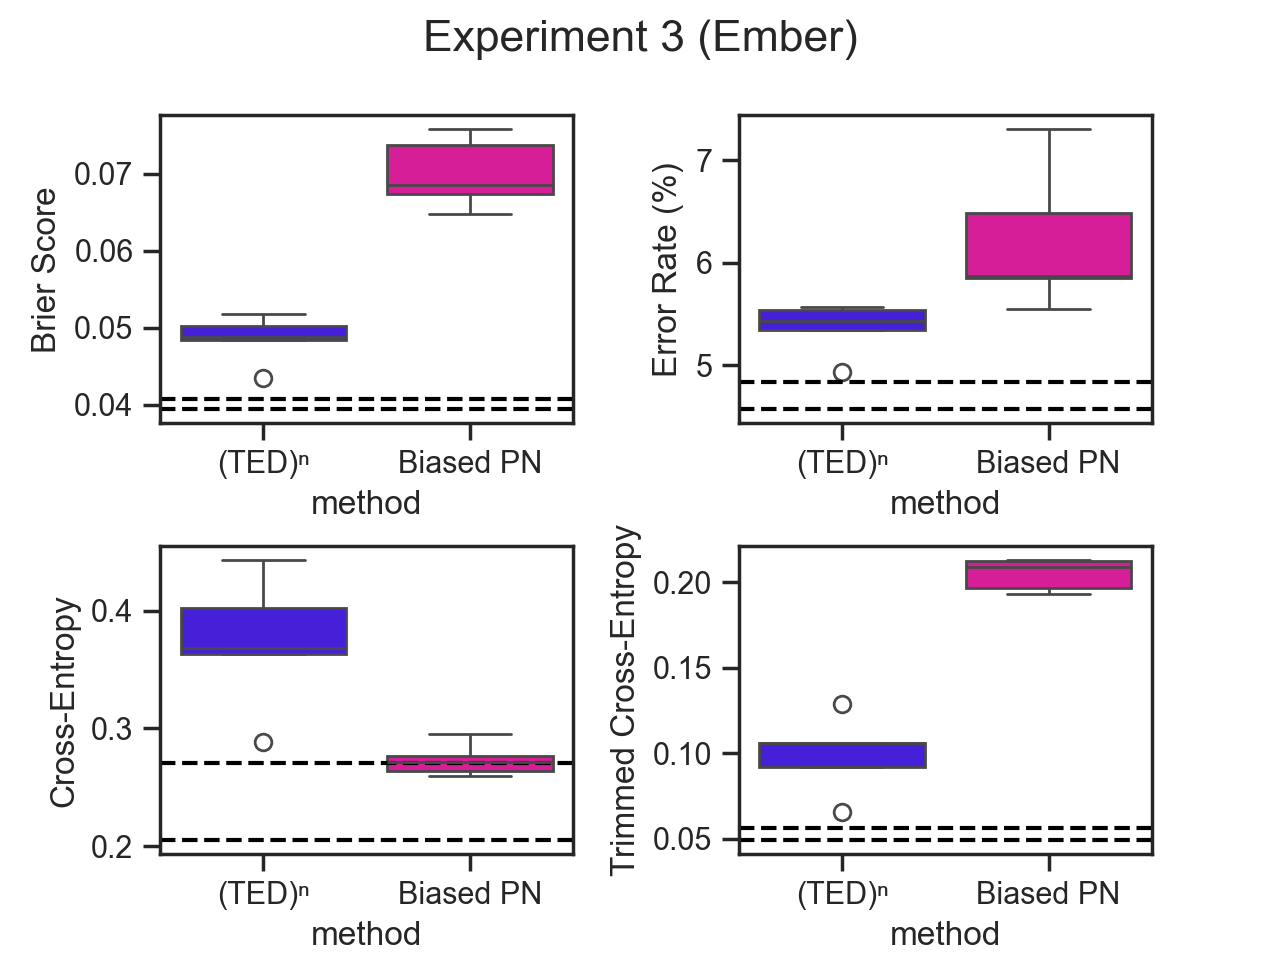
\includegraphics[scale=0.5]{experiment-3}
        \caption{Test-set metrics for experiment 3.} 
        \label{fig:exp3} 
    \end{figure*} 

    Experiment 3 compares the performance of the (TED)${}^n$ method and the biased PN model using the \textsc{ember} dataset's 300,000 unlabeled data directly. We create a synthetic unlabeled dataset by combining the unlabeled data with the negative data. This adds some (unknown) number of positive samples to the unlabeled data \textit{without} reducing the number of positive labels among the training data. Adding these unlabeled samples to the negative set likewise increases the total number of negatives available in the training data, as there are presumably some number of negative examples among the unlabeled data. This is a key difference between Experiment 3 and Experiments 1 and 2. In Experiments 1 and 2, each positive sample moved into the unlabeled set decreased the number of positive labels available to the model, but the number of negatives remained the same. This experiment uses the same model architecture and hyper-parameters as Experiment 2.

    Figure \ref{fig:exp3} shows the results of Experiment 3. Similarly to Experiment 2, the (TED)${}^n$ method shows lower Brier score and trimmed cross-entropy. The error rates between the two methods are comparable, although the (TED)${}^n$ error rates are more tightly clustered around a smaller median than the biased PN model's. According to Brier score and trimmed cross-entropy, the (TED)${}^n$ model is strongly preferred to the biased PN model.

    However, the cross-entropy values are consistently worse for the (TED)${}^n$ model, as they were in Experiment 2. We attribute this finding to the same mechanism as before, in which the the (TED)${}^n$ model's higher average values of cross-entropy are driven by the presence of outliers which exert large influence on the mean. The omission of extreme values reveals that, for the vast majority of observations, the (TED)${}^n$ model is preferred.

    We statistically test the differences in each of the four metrics; the $t$ values are reported in table \ref{tab:exp3}. As with Experiment 2, we find that the Brier score and trimmed cross-entropy show a statistically significant difference, while the cross-entropy and error rate do not. That said, the $p$-value of the error rate is 0.053, which is not significant at the 5\% level.

\section{Discussion}
\label{sec:discuss}

    In all cases, the most pronounced improvements in model quality occur when there is a larger proportion of positives among the unlabeled data. This is intuitive -- when the proportion of labeling errors is smaller, the labeling errors will have a smaller influence on what the model learns. Future work should attempt to understand the prevalence of labeling errors in different sources of threat intelligence (e.g. VirusTotal, Hybrid Analysis, Recorded Future). Also, discovering common factors among the errors may allow a determination of root cause or systematic omissions in how labels are assigned, improving the quality of threat feeds overall.

    The DGA results demonstrate that the (TED)${}^n$ procedure can be extremely effective. The results for the DGA task demonstrate a nearly uniform improvement to models in the PU setting. We attribute this success to the overall effectiveness of the modeling strategy: 3-grams are tremendously informative as a method for detecting randomized domain name strings. Therefore, the (TED)${}^n$ procedure is easily able to remove positives from among the unlabeled data.

    On the other hand, the mixed results of the (TED)${}^n$ method when applied to the textsc{ember} dataset suggests that the effectiveness of (TED)${}^n$ depends strongly on the underlying model. In Anderson \& Roth's original publication, they report a ROC AUC of 0.99911 for a gradient boosted tree model trained on the \textsc{ember} data. Our benchmark model only obtains ROC AUC 0.984 (the mean of 5-fold cross validation) and a 95\% confidence interval of [0.9831, 0.9849]. So the model that we used in this study is substantially worse than the Anderson \& Roth model, and using a model with comparable effectiveness may alter these results.

    We conjecture several potential causes our neural network model's poor performance.
    \begin{itemize}
        \item We use 5-fold cross-validation of the training data to construct a validation set used for early stopping (in PN models) and to estimate mixture proportion (for (TED)${}^n$ models). The 20\% reduction in training data size could impair model effectiveness.
        \item Anderson \& Roth used gradient boosted decision trees. Perhaps this finding is further evidence that multi-layer perceptrons are less effective than gradient boosted decision trees on tabular data. (This is a widely-acknowledged phenomenon; for example, \cite{armon-2022}).
        \item The \textsc{ember} code is a few years out of date, so we were forced to use newer library versions and kludge a few lines of code. This may have changed the value of the feature vectors in a way that impairs the model.
    \end{itemize}

\section{Conclusion}
\label{sec:conclude}

    These results demonstrate that the (TED)${}^n$ procedure can reduce the bias arising from building models with PU data. These improvements in model quality are often statistically significant and reduce the number of errors (false positives, false negatives) that the model makes. 

    Future work should study the efficacy of the (TED)${}^n$ procedure in conditions that are closer to the real-world setting of industry practitioners. Both datasets are very small by the standards of industry. An industrial-scale machine learning model for computer security would use hundreds of millions to billions of samples. The DGA dataset has 1.4 million samples and the \textsc{ember} dataset has 1.1 million samples. Collecting more data is often the shortest path to improving model quality, and the (TED)${}^n$ procedure removes one of the largest costs to exploiting that data, access to benign labels.

    While these methods have demonstrated some effectiveness on small-scale computer security problems, the real challenge is to assess the benefits and drawbacks of PU learning generally, and (TED)${}^n$ specifically, in real-world industrial security applications. Certainly, one component of that is increasing the size of the datasets. A second component is accounting for the sequential nature of the problem, where new objects and labels arrive over time (possibly with labels arriving some time after the sample itself). A third component is identifying how and when adversarial actions to manipulate classification decisions (e.g. data poisoning). A fourth is to develop a deeper understanding of the failure modes for PU learning, and how to remedy them. These improvements would improve enhance computer security by enabling full use of the enormous volumes of unlabeled data which characterize the computer security industry.

\bibliographystyle{ieeetran}
\bibliography{camlis-2024-bibliography} % without .bib extension

\appendix

\subsection{Model Hyperparameters}
\label{appendix:hyperparams}
    All model training is done in PyTorch. Full code is available in the Github repository. These model configurations were not tuned because we desire a like-to-like comparison between the Biased PN method and (TED)${}^n$, and to eliminate model selection as a possible source of confounding in the results. It's plausible that better models exist.

    Table \ref{tab:dga-hyper} presents the DGA model's configuration details. 

    \begin{table}
    \caption{Hyper-parameters for DGA model}
    \label{tab:dga-hyper}
        \begin{tabular}{l | l }
            batch size & 2048 \\
            warmup epochs & 1 \\
            number of residual blocks & 3 \\
            number of stride 1 convolution blocks & 1 \\
            embedding dimension & 16 \\
            model dimension & 256 \\
            optimizer & AdamW $(\beta_1 = 0.9,~\beta_2 = 0.999)$ \\
            weight decay & 0 \\
            learning rate & $10^{-4}$ \\
            learning rate scheduler & \texttt{StepLR} \\
            learning rate scheduler step size & 0.5 \\
            learning rate schedule $\gamma$ & 4 \\
            early stopping patience & 3 epochs \\
            BBE $\gamma$ hyper-parameter & 0
        \end{tabular}
    \end{table}

    Table \ref{tab:ember-hyper} presents the \textsc{ember} model's configuration details.

    \begin{table}
    \caption{Hyper-parameters for \textsc{ember} model}
    \label{tab:ember-hyper}
        \begin{tabular}{l | l }
            batch size & 1024 \\
            warmup epochs & 4 \\
            number of residual blocks & 3 \\
            model dimension & 512 \\
            optimizer & AdamW $(\beta_1 = 0.9,~\beta_2 = 0.999)$ \\
            weight decay & 0 \\   
            learning rate & $3 \times 10^{-4}$ \\
            learning rate scheduler & \texttt{StepLR} \\
            learning rate scheduler step size & 0.75 \\
            learning rate schedule $\gamma$ & 4 \\
            early stopping patience & 8 epochs \\
            BBE $\gamma$ hyper-parameter & 0
        \end{tabular}
    \end{table}

\subsection{Statistical Results}
\label{appendix:tables}

    In each table, the $t$ statistic has a star if it is significant at the 5\% level. For all experiments, the $t$-statistic has $\frac{5}{2}-1=1.5$ degrees of freedom.

    The benchmarks and experiments are repeated using 5-fold cross validation, where the hold-out set of the validation data is used to compute BBE (for (TED)${}^n$) or the early-stopping criterion (for PN training).

    Experiment 3 only has 1 row because the number of unlabeled is fixed by the \textsc{ember} dataset: the unlabeled set is the combination of \textsc{ember}'s unlabeled data plus all of \textsc{ember}'s negative data. (This experiment allows us to make a comparison where all available positive labels are in the positive set; the other experiments remove positive labels to construct the unlabeled set.)

    \begin{table}
    \caption{Experiment 1 (DGA) $t$ statistics}
    \label{tab:exp1}
        \begin{tabular}{r | r | r | r | r}
            \hline
                \makecell{Percent \\ Positives \\ Relabeled}
                & Brier score & cross-entropy & error rate & \makecell{trimmed \\ cross-entropy} \\
            \hline                                                    
                0.05  &           -5.02 *  &     -1.30~~~&   -3.78 *  &         -34.81 *\\
                0.10  &          -13.09 *  &     -9.68 * &   -5.99 *  &         -72.51 *\\
                0.15  &          -35.81 *  &    -14.54 * &  -14.55 *  &         -81.93 *\\
                0.20  &          -39.49 *  &    -31.91 * &   -8.65 *  &         -84.00 *\\
                0.25  &          -27.47 *  &    -32.42 * &   -5.01 *  &         -49.06 *\\
                0.30  &          -34.40 *  &    -30.86 * &   -6.13 *  &         -84.75 *\\
                0.35  &          -80.23 *  &    -38.79 * &   -8.74 *  &        -325.36 *\\
                0.40  &          -50.24 *  &    -52.96 * &   -7.24 *  &        -117.30 *\\
                0.45  &          -82.76 *  &    -62.60 * &  -13.48 *  &        -140.61 *\\
                0.50  &         -109.33 *  &    -62.51 * &  -34.81 *  &        -155.96 *\\
                0.55  &         -183.04 *  &    -54.92 * &  -88.50 *  &        -237.70 *
        \end{tabular}
    \end{table}

    \begin{table}[!h]
    \caption{Experiment 2 (Ember) $t$ statistics}
    \label{tab:exp2}
        \begin{tabular}{r | r | r | r | r}
            \hline
                \makecell{Percent \\ Positives \\ Relabeled}
                & Brier score & cross-entropy & error rate & \makecell{trimmed \\ cross-entropy} \\
            \hline                                                    
                0.05  &   4.94~~~  & 20.37 &   -1.74~~~  &  0.75~~~ \\
                0.10  &   1.30~~~  &  9.26 &   -2.42 *   & -6.96 * \\
                0.15  &  -2.07~~~  & 11.29 &   -0.76~~~  & -6.45 * \\
                0.20  &  -4.31 *   &  3.62 &   -0.66~~~  & -2.72 * \\
                0.25  &  -4.77 *   &  6.02 &   -0.50~~~  & -3.10 * \\
                0.30  &  -6.08 *   &  6.62 &   -0.20~~~  & -3.63 * \\
                0.35  &  -9.40 *   &  3.81 &   -1.24~~~  & -2.65 * \\
                0.40  & -10.91 *   &  2.86 &   -2.72 *   & -4.73 * \\
                0.45  & -11.52 *   &  3.54 &   -3.31 *   & -4.20 * \\
                0.50  & -32.72 *   &  8.47 &   -5.50 *   & -4.19 * \\
                0.55  & -74.99 *   &  5.39 & -141.65 *   & -3.99 *
        \end{tabular}
    \end{table}

    \begin{table}
    \caption{Experiment 3 (Ember with unlabeled data) $t$ statistics}
    \label{tab:exp3}
        \begin{tabular}{r | r | r | r}
            \hline
                Brier score & cross-entropy & error rate & \makecell{trimmed \\ cross-entropy} \\
            \hline                                                    
            -7.53 * & 3.36 & -2.08 & -9.33 *
        \end{tabular}
    \end{table}

\end{document}